\documentclass[12pt]{extarticle}
%Some packages I commonly use.
\usepackage[english]{babel}
\usepackage{graphicx}
\usepackage{framed}
\usepackage[normalem]{ulem}
\usepackage{amsmath}
\usepackage{amsthm}
\usepackage{amssymb}
\usepackage{amsfonts}
\usepackage{enumerate}
\usepackage[utf8]{inputenc}
\usepackage{listings}
\usepackage[top=1 in,bottom=1in, left=1 in, right=1 in]{geometry}
\usepackage{color}
\usepackage{float}

\definecolor{dkgreen}{rgb}{0,0.6,0}
\definecolor{gray}{rgb}{0.5,0.5,0.5}
\definecolor{mauve}{rgb}{0.58,0,0.82}

%A bunch of definitions that make my life easier
\newcommand{\matlab}{{\sc Matlab} }
\newcommand{\cvec}[1]{{\mathbf #1}}
\newcommand{\rvec}[1]{\vec{\mathbf #1}}
\newcommand{\ihat}{\hat{\textbf{\i}}}
\newcommand{\jhat}{\hat{\textbf{\j}}}
\newcommand{\khat}{\hat{\textbf{k}}}
\newcommand{\minor}{{\rm minor}}
\newcommand{\trace}{{\rm trace}}
\newcommand{\spn}{{\rm Span}}
\newcommand{\rem}{{\rm rem}}
\newcommand{\ran}{{\rm range}}
\newcommand{\range}{{\rm range}}
\newcommand{\mdiv}{{\rm div}}
\newcommand{\proj}{{\rm proj}}
\newcommand{\R}{\mathbb{R}}
\newcommand{\N}{\mathbb{N}}
\newcommand{\Q}{\mathbb{Q}}
\newcommand{\Z}{\mathbb{Z}}
\newcommand{\<}{\langle}
\renewcommand{\>}{\rangle}
\renewcommand{\emptyset}{\varnothing}
\newcommand{\attn}[1]{\textbf{#1}}
\theoremstyle{definition}
\newtheorem{theorem}{Theorem}
\newtheorem{corollary}{Corollary}
\newtheorem*{definition}{Definition}
\newtheorem*{example}{Example}
\newtheorem*{note}{Note}
\newtheorem{exercise}{Exercise}
\newcommand{\bproof}{\bigskip {\bf Proof. }}
\newcommand{\eproof}{\hfill\qedsymbol}
\newcommand{\Disp}{\displaystyle}
\newcommand{\qe}{\hfill\(\bigtriangledown\)}
\setlength{\columnseprule}{1 pt}

\lstset{frame=tb,
	language=C,
	aboveskip=3mm,
	belowskip=3mm,
	showstringspaces=false,
	columns=flexible,
	basicstyle={\small\ttfamily},
	numbers=none,
	numberstyle=\tiny\color{gray},
	keywordstyle=\color{blue},
	commentstyle=\color{dkgreen},
	stringstyle=\color{mauve},
	breaklines=true,
	breakatwhitespace=true,
	tabsize=3
}

\title{CS307 Project1: Introduction To Linux Kernel Module}
\author{Junjie Wang 517021910093}

\begin{document}

	\maketitle
	\section{Programming Thoughts}
	\subsection{Part 1}
	In the first part, first we have to create an initilization function and exiting function for our kernel module. Then we need to include necessary header files(e.g. linux/jiffies.h linux/gcd.h) to use the global variables and functions which are only available in kernel space. Another thing worth attention is the different types for these variables.  
	\subsection{Part 2}
	In the second part, we need to interact with the /proc pseudo file system. First we need to print out the value of jiffies variable in $proc\_read()$ function and then we need to use this equation to get the time interval.
	$$t = \frac{jiffies_t - jiffies_0}{HZ} $$
	\section{Execution Results And Snapshots}
	The execution results are shown in \ref{fig1} and \ref{fig2}.
	\begin{figure}[H]
	\centering 
	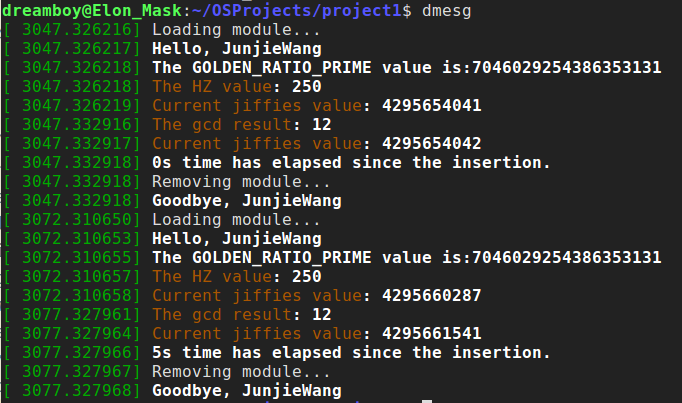
\includegraphics[width=0.8\textwidth]{../imgs/1-1.png}
	\caption{part 1}
	\label{fig1}
	\end{figure}
	\begin{figure}[htbp]
	\centering
	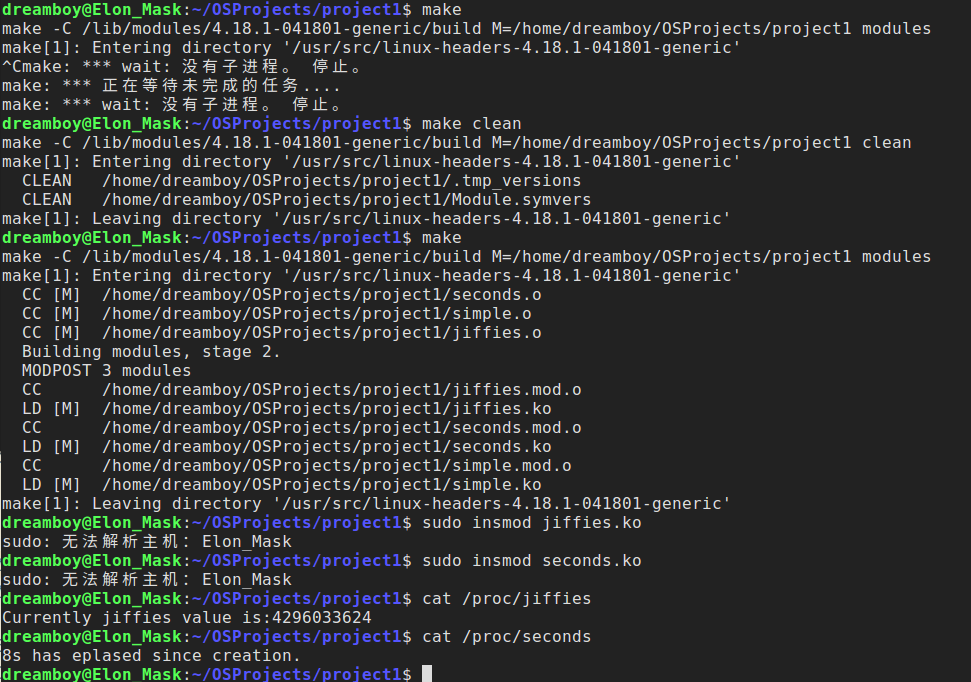
\includegraphics[width=0.8\textwidth]{../imgs/1-2.png}
	\caption{part 2}
	\label{fig2}
	\end{figure} 
	\section{Code Explanation}
	The $proc\_init()$ and $proc\_read()$ are shown as belows. We first use a global variable \textbf{start} to record the value of jiffies at the beginning. And then use the formula to get the time interval when the $proc\_read()$ function is invoked.
	\begin{lstlisting}
		static int proc_init(void)
		{
		proc_create(PROC_NAME, 0666, NULL, &proc_ops);
		printk(KERN_INFO "/proc/%s created\n", PROC_NAME);
		start = jiffies;
		
		return 0;
		}
		...
		static ssize_t proc_read(struct file *file, char __user *usr_buf, size_t count, loff_t *pos)
		{
		int rv = 0;
		static int completed = 0;
		char buffer[BUFFER_SIZE];
		
		if(completed){
		completed = 0;
		return 0;
		}
		
		completed = 1;
		
		rv = sprintf(buffer, "%lus has eplased since creation.\n", (jiffies-start)/HZ);
		
		copy_to_user(usr_buf, buffer, rv);
		return rv;
		}
	\end{lstlisting}
		
	\end{document}